\documentclass[../main.tex]{subfiles}

\begin{document}
\section{Challenges and lessons learned} \label{sec:challenges}
Several significant challenges were faced throughout the project, which we reflect on in this section as a reference for potential future work on the Raspberry Pi camera array.

\subsection{Camera array power setup} \label{sec:challenges-power}
A significant challenge which presented itself early in the project was the camera array's power setup. Initially, not all Raspberry Pi devices were powering on. This meant that at the start of the project, the cause of the failing Raspberry Pis needed to be identified and fixed. The power setup and lack of cable management meant that identifying the cause was a significant problem itself (see figure~\ref{fig:cable-management}). A failing Raspberry Pi was also noted in Denham's technical report \cite{denhamRaspberry}.

\begin{figure}[H]
    \centering
    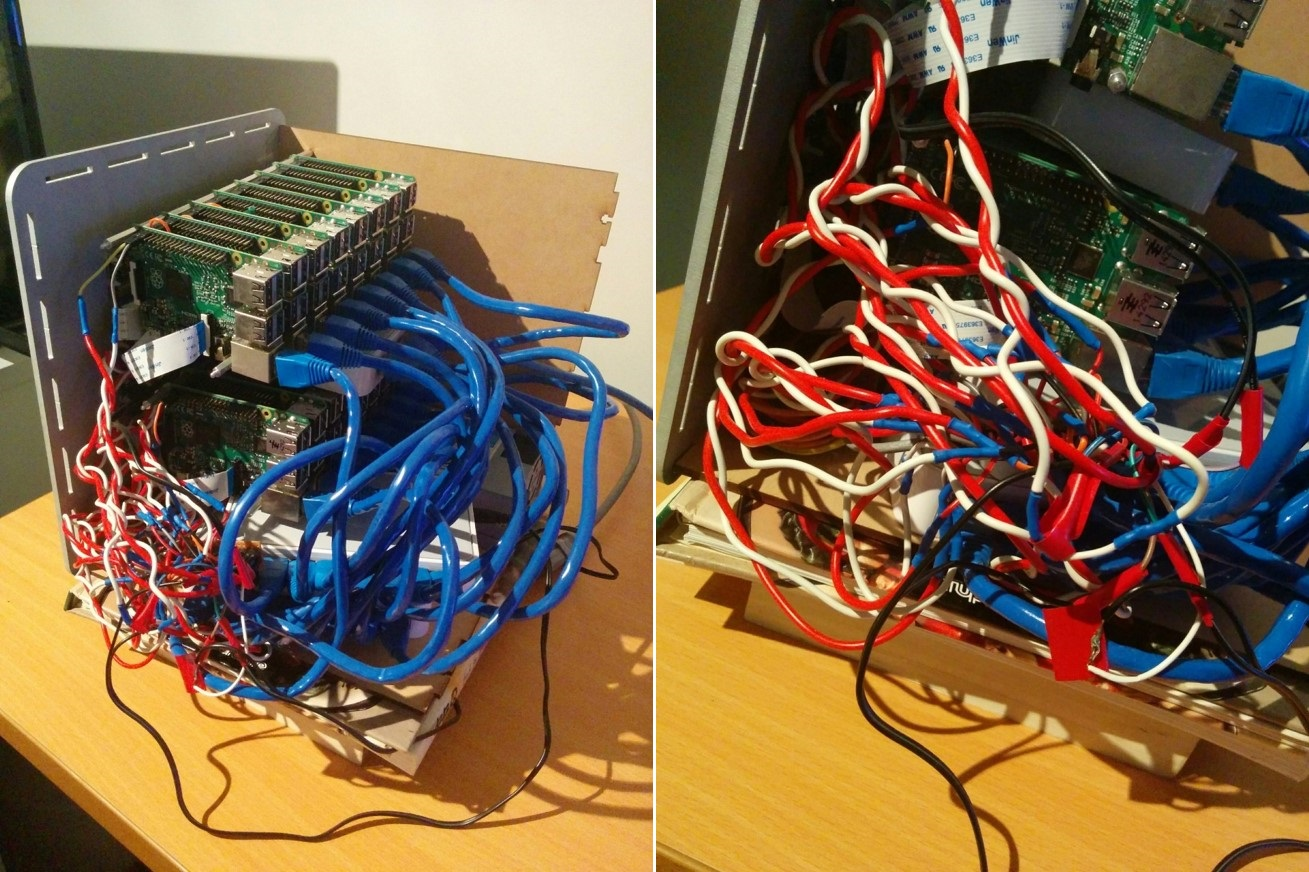
\includegraphics[width=\linewidth]{images/cable-management}
    \caption{Raspberry Pi camera array power setup. Notice the poor cable management.}
    \label{fig:cable-management}
\end{figure}

Solving the problem required the camera array to be pulled apart and reconstructed, ensuring all cables were plugged in securely. Unfortunately, the power setup was also extremely temperamental - power cables frequently came loose, and often required resoldering. As soldering was a new skill, training and practice was required.

Once all cameras were powering on and had the right software, such issues were relatively infrequent. For future work, it may prove beneficial to redesign the power setup of the array, so that cables are organised, safe and secure. 

\subsection{Camera array hardware setup} \label{sec:challenges-power}
The way Raspberry Pis are positioned within the enclosure makes it difficult to access SD cards, power cables and camera board cables (see figure~\ref{fig:hardware-access}). If SD cards need re-imaging, or power or camera board cables need resitting, the entire array may need to be pulled apart. 

\begin{figure}[H]
    \centering
    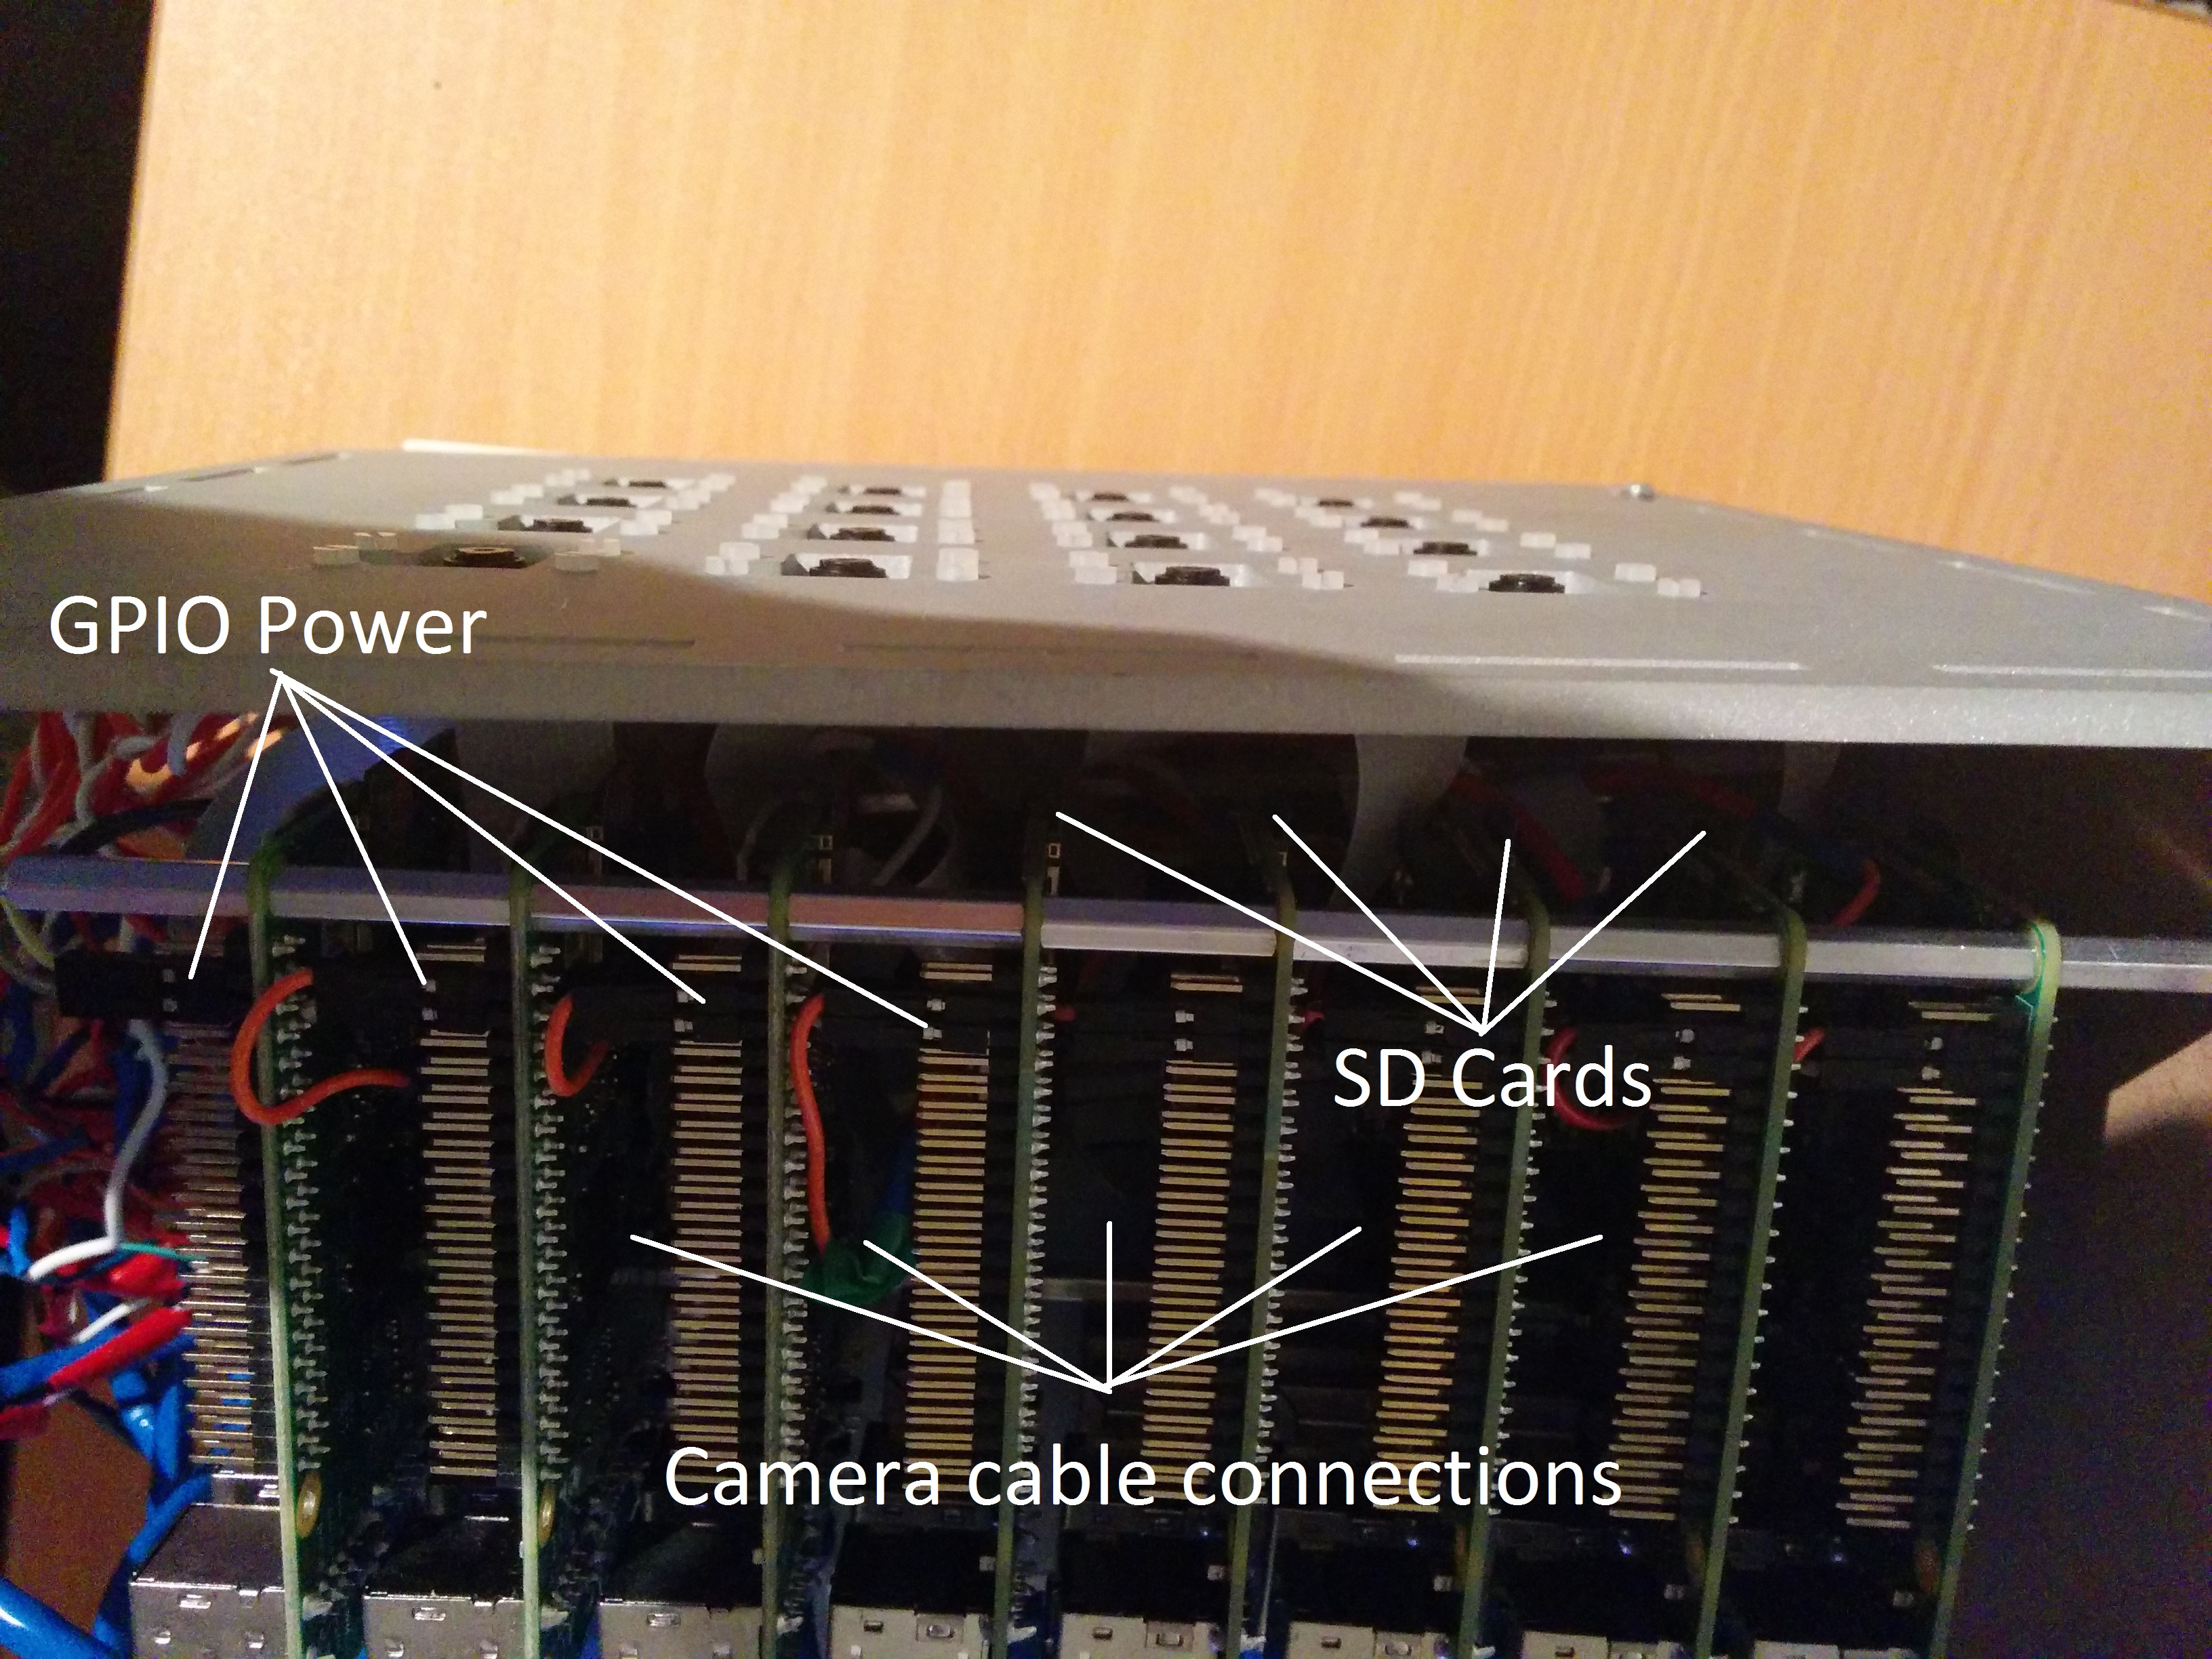
\includegraphics[width=0.75\linewidth]{images/hardware-access}
    \caption{Top-down view of the camera array enclosure with the top removed. Key areas requiring regular access are labelled. It is difficult to access these areas without deconstructing the array of Raspberry Pis.}
    \label{fig:hardware-access}
\end{figure}

Again, once the camera array has all the necessary software and all cables are secure, these issues do not cause serious problems. Nevertheless, we highly recommend redesigning the enclosure so that Raspberry Pis are not situated as they are presently.

\subsection{Raspberry Pi software setup}
In the early stages of the project, we wanted to demonstrate camera function via a live video stream to each Raspberry Pi camera module. It was discovered that the MATLAB support package for Raspberry Pi devices could achieve this. However, this requires Raspberry Pis to be set up with MATLAB's Raspbian distribution, since MathWorks does not provide the streaming software on its own. Setting up the new OS was a tedious process, because it required that the entire camera array be pulled apart so that SD cards could be retrieved, imaged, and put back into place.

After successfully testing camera functionality via live streams through MATLAB, our aim was to capture synchronised images and video. In Denham's original report, CompoundPi is suggested for synchronised capture. Installing the CompoundPi software package presented another challenge, since software needed to be downloaded and configured across Raspberry Pi devices. Since only one device can be connected to Wi-Fi at a time (we only have one Wi-Fi dongle), we attempted to install and configure CompoundPi on one device to start with. At this point, it was discovered that CompoundPi was incompatible with MATLAB's Raspbian distribution, so we decided to revert to a plain Raspbian distribution. Once we had one Raspberry Pi working with pure Raspbian and CompoundPi, we pulled apart the array to copy the image to the other 15 devices and reconstruct the array.

Later, we discovered that CompoundPi does not support synchronised video well. After some exploration, we found that the \emph{SuperPutty} software package for Windows could synchronise commands to many devices via SSH. This could effectively replace CompoundPi so that we can capture synchronised images and video using the default capture commands \texttt{raspistill} and \texttt{raspivid}, without requiring any third-party software. This is our current software recommendation.

\end{document}